\documentclass[conference]{IEEEtran}
\IEEEoverridecommandlockouts
% Based on the IEEE conference template (version 6/27/2024).

\usepackage{cite}
\usepackage{amsmath,amssymb,amsfonts}
\usepackage{algorithmic}
\usepackage{graphicx}
\usepackage{textcomp}
\usepackage{xcolor}
\usepackage{url}
\graphicspath{{figures/}}
\def\BibTeX{{\rm B\kern-.05em{\sc i\kern-.025em b}\kern-.08em
    T\kern-.1667em\lower.7ex\hbox{E}\kern-.125emX}}

\begin{document}

\title{Deadlock Detection and Prevention in Business Process Models Using Petri Nets}

\author{\IEEEauthorblockN{Devansh Rai}
\IEEEauthorblockA{\textit{Dept. of Information Technology} \\
\textit{Indian Institute of Information Technology Allahabad}\\
Prayagraj, India \\
iib2024006@iiita.ac.in}
\and
\IEEEauthorblockN{Geethika Gorakala}
\IEEEauthorblockA{\textit{Dept. of Information Technology} \\
\textit{Indian Institute of Information Technology Allahabad}\\
Prayagraj, India \\
iib2024024@iiita.ac.in}
\and
\IEEEauthorblockN{Abhilasha Sharma}
\IEEEauthorblockA{\textit{Dept. of Information Technology} \\
\textit{Indian Institute of Information Technology Allahabad}\\
Prayagraj, India \\
iib2024501@iiita.ac.in}
}

\maketitle

\begin{abstract}
A BPMN model can pass a visual review and still contain a state in which a running case stops before it
reaches its end. We present a tool that finds such deadlocks, explains them and repairs the model. It reads a
BPMN 2.0 file, maps it to a workflow Petri net, searches the diagram for six known error patterns and explores
the full state space to check soundness and safeness. Every dead state is reported together with the sequence of
steps that leads to it. Circular waits on shared resources are traced to empty siphons and prevented with a
control place, and gateway errors are corrected in the BPMN file itself. The repaired model is then analysed
again. We tested the tool on 16 models: eleven from a loan approval process, including a complex model with
five defects, and five from other domains. All eight faulty models were repaired and verified as sound, and our
verdicts agree with the pm4py soundness checker on every model. In the complex model the first defects stopped
every case early, so two of the remaining defects only became visible after the first fixes. None of the
control places blocked a state from which the process could still finish. The tool is available as a web
application.
\end{abstract}

\begin{IEEEkeywords}
BPMN, Petri nets, deadlock, soundness, siphon, deadlock prevention, process verification
\end{IEEEkeywords}

\section{Introduction}
Consider a loan application process. After the application is received, the bank runs a credit check and a
document check in parallel, and an AND-join waits for both before the decision is made. If the documents are
incomplete, the document branch moves the application to ``on hold'', and that task has no outgoing flow. The
AND-join now waits for a document result that never arrives, and the application is neither approved nor
rejected. Nothing in the diagram looks wrong at first glance. Every element is drawn correctly; the error lies
in how the elements behave together.

BPMN~\cite{bpmn} is the usual notation for such processes. It is easy to read, but its behaviour is described
informally, so errors of this kind are found late, often when a case is already stuck~\cite{kraeuter,zhang}.
Petri nets give the same process a precise meaning~\cite{murata}. Once a BPMN model is mapped to a Petri net, a
deadlock is a reachable state in which no transition can fire although the case has not finished, and such
states can be found by a search. For the person who drew the model, a list of stuck states is only half an
answer. They also need to know which element caused the problem and how to change it, and in processes with
shared staff or systems the cause may be a circular wait rather than a wrong gateway.

This paper asks how Petri nets can be used to detect and prevent deadlocks in business process models while
keeping the behaviour that already worked. Our contributions are:
\begin{enumerate}
\item a six-step framework that goes from a BPMN model to a verified corrected model, with re-analysis after
every fix;
\item a Python tool that combines the soundness and safeness checks and quick fixes of Kr\"auter
et al.~\cite{kraeuter}, the mapping and change checks of Zhang et al.~\cite{zhang} and the siphon-based
prevention of Wang et al.~\cite{wang}, and adds shared resources and a timed simulation;
\item a case study of eleven loan approval models, including a complex model with five interacting defects
that is repaired over three rounds, and five models from other domains;
\item an evaluation against an independent checker, a scalability benchmark and a measure of how much
behaviour each repair keeps.
\end{enumerate}

Section~II reviews related work and Section~III gives the definitions we use. Section~IV describes the six
steps and Section~V the implementation. Section~VI reports the results, Section~VII discusses them and
Section~VIII concludes.

\section{Related Work}

\subsection{Soundness Checking of BPMN Models}
Kr\"auter et al.~\cite{kraeuter} built a soundness checker for BPMN that runs inside the bpmn.io modeller.
It explores the whole state space with a breadth-first search and checks option to complete, proper
completion, no dead activities and safeness during the search. A task is encoded as a single step instead of a
separate start and end, which keeps the state space small; on their benchmarks the checker answers in a few
milliseconds. The tool highlights the elements involved in a violation, replays the counterexample as moving
tokens and offers quick fixes in the style of an IDE. For a split and join that do not match, it proposes
two fixes, one at the join and one at the split, and the modeller picks one. The checker does not handle data,
time or shared resources.

\subsection{Formal Mapping and Model Evolution}
Zhang et al.~\cite{zhang} map BPMN collaboration models to hierarchical coloured Petri nets. Colour sets carry
business objects, and sub-processes become substitution transitions with ports. Their Algorithm~1 checks that
every BPMN element and connection has a counterpart in the net, and their Algorithm~2 compares two versions of
a model and lists the changes as insert, delete and replace operations. Each evolved model is verified with a
state-space report from CPN Tools. Their evaluation covers two small examples and does not address deadlock
prevention beyond a short list of ideas.

\subsection{Siphon-Based Deadlock Prevention}
Wang et al.~\cite{wang} study Petri nets in which every resource place starts with exactly one token. A
mixed-integer program finds a particular class of emptiable siphons, which avoids both listing all siphons and
building the reachability graph. A control place with unit arc weights is then added for each such siphon. The
resulting controller is maximally permissive: it forbids only the states that lead to a deadlock.

\subsection{Our Position}
None of these works covers the whole path from a BPMN diagram with shared resources to a repaired and
re-verified model. We take the state-space checks and quick fixes of~\cite{kraeuter}, the mapping and change
checks of~\cite{zhang} without colours and hierarchy, and the control-place construction of~\cite{wang}
without the mixed-integer program. Correctness is judged by the soundness of workflow nets as defined by
van der Aalst~\cite{aalst}.

\section{Preliminaries}

\textbf{Petri net.} A Petri net is a tuple $N=(P,T,F,W)$ with finite disjoint sets of places $P$ and
transitions $T$, arcs $F\subseteq(P\times T)\cup(T\times P)$ and arc weights $W:F\to\mathbb{N}^+$. A marking
$M:P\to\mathbb{N}$ assigns a number of tokens to each place. A transition $t$ is enabled in $M$, written
$M[t\rangle$, if $M(p)\ge W(p,t)$ for every input place $p\in{}^\bullet t$. Firing $t$ gives the marking $M'$
with
\begin{equation}
M'(p)=M(p)-W(p,t)+W(t,p)\quad\text{for all }p\in P.
\end{equation}
$R(N,M_0)$ is the set of markings reachable from the initial marking $M_0$.

\textbf{Workflow net.} A workflow net has one source place $i$ and one sink place $o$. A case starts with
$M_0=[i]$ and should end in $M_f=[o]$. In our nets, a shared resource is a place that holds its free units;
these units are present in both $M_0$ and $M_f$.

\textbf{Deadlock.} A marking $M\in R(N,M_0)$ is dead if no transition is enabled. A dead marking other than $M_f$
is a deadlock if the sink is empty and an improper completion if it is not. Formally, a marking $M$ with
\begin{equation}
M\in R(N,M_0),\qquad M\neq M_f,\qquad \nexists\, t\in T: M[t\rangle
\end{equation}
is a deadlock if $M(o)=0$ and an improper completion if $M(o)\ge 1$.

\textbf{Soundness}~\cite{aalst}. A workflow net is sound if (1) $M_f$ can be reached from every reachable
marking (option to complete), (2) no reachable marking marks $o$ while other tokens remain (proper completion),
and (3) every transition fires in at least one run (no dead transitions). Following~\cite{kraeuter} we also
check \emph{safeness}: no place that represents a sequence flow ever holds more than one token. An unsafe flow
usually means a missing synchronisation.

\textbf{Siphon}~\cite{wang,murata}. A non-empty set $S\subseteq P$ is a siphon if
${}^\bullet S\subseteq S^\bullet$: every transition that puts a token into $S$ also takes one from $S$. Once a
siphon is empty it stays empty, and every transition that needs one of its places can never fire again. An
empty siphon is the signature of a circular wait.

\section{Proposed Methodology}
Fig.~\ref{fig:framework} shows the six steps. A corrected model goes back through steps 2 and 3 and is
accepted only when it is sound.

\begin{figure}[htbp]
\centerline{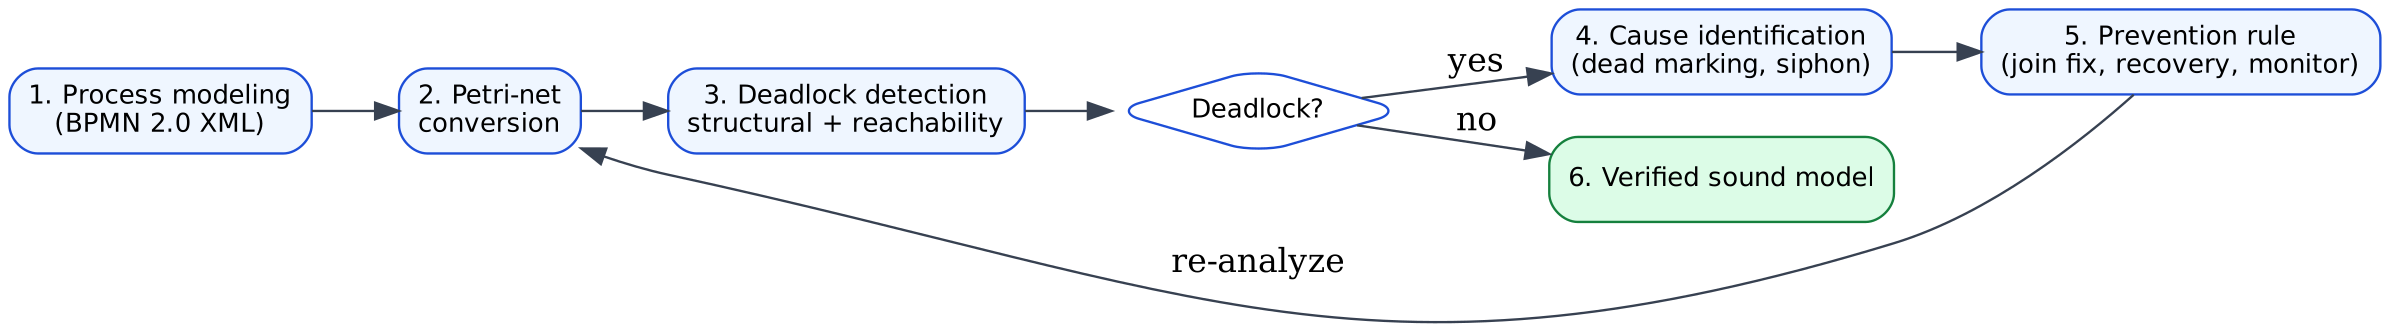
\includegraphics[width=\columnwidth]{framework.png}}
\caption{The six steps of the framework. A fixed model returns to the analysis.}
\label{fig:framework}
\end{figure}

\subsection{Step 1: Process Modelling}
Models are drawn in BPMN 2.0 with Camunda Modeler or bpmn.io and saved as XML. Information that BPMN has no
field for is written in the standard documentation field, so the files remain valid BPMN: the process lists its
resources (\texttt{resources: officer=1}), a task states its duration and the resources it takes or releases
(\texttt{time: 20; acquire: officer}), and a sequence flow leaving an XOR gateway states its probability
(\texttt{prob: 0.3}).

\subsection{Step 2: Mapping to a Petri Net}
Table~\ref{tab:map} gives the mapping. It follows the element rules of Zhang et al.~\cite{zhang} without colours
and hierarchy. Like~\cite{kraeuter}, a task is a single transition. Every sequence flow becomes its own place,
so any token in the net can be traced back to an arrow in the diagram. After the mapping, the check
of~\cite{zhang} (Algorithm~1) confirms that every BPMN element has at least one transition, that every sequence
flow has a place, and that this place is produced by the flow's source and consumed by its target.

\begin{table}[htbp]
\caption{Mapping from BPMN to Petri Net}
\begin{center}
\begin{tabular}{|p{0.30\columnwidth}|p{0.58\columnwidth}|}
\hline
\textbf{BPMN element} & \textbf{Petri net pattern} \\
\hline
Sequence flow & one place \\
Start event & source place $i$ with one token and a transition \\
End event & a transition into the sink place $o$ \\
Task & one transition from its input place to its output place \\
AND-split, AND-join & one transition with several output or input arcs \\
XOR-split, XOR-join & one transition per outgoing or incoming branch \\
OR-split & one transition per non-empty subset of branches \\
Shared resource & a place with its free units; \emph{acquire} adds an input arc, \emph{release} an output arc \\
Element without outgoing flow & a ``stuck'' place that nothing consumes \\
\hline
\end{tabular}
\label{tab:map}
\end{center}
\end{table}

\subsection{Step 3: Deadlock Detection}
\emph{Structural check.} Kr\"auter et al.~\cite{kraeuter} list typical causes for each soundness violation: a
parallel join that waits for branches that never all arrive, an exclusive join that merges parallel branches,
an activity that cannot be reached. They look for the cause after a counterexample has been found. We search
the BPMN graph for these causes before any state is explored, as the six patterns in Table~\ref{tab:patterns}.
For P1, the tool walks forward from every branch of the split. The pattern holds if one branch reaches an
incoming flow $a$ of the join but not another incoming flow $b$, while a second branch reaches $b$ but not $a$.

\begin{table}[htbp]
\caption{Error Patterns of the Structural Check}
\begin{center}
\begin{tabular}{|c|p{0.47\columnwidth}|p{0.29\columnwidth}|}
\hline
\textbf{Code} & \textbf{Pattern} & \textbf{Property broken} \\
\hline
P1 & XOR- or OR-split closed by an AND-join & option to complete \\
P2 & AND-join at the entry of a loop & option to complete \\
P3 & AND-split closed by an XOR-join & safeness, proper completion \\
P4 & element without outgoing flow & option to complete \\
P5 & element that cannot be reached & no dead transitions \\
P6 & two resources taken in opposite orders & option to complete \\
\hline
\end{tabular}
\label{tab:patterns}
\end{center}
\end{table}

\emph{State-space analysis.} A breadth-first search builds the reachability graph from $M_0$ and stores, for
each new marking, the marking and transition it was reached from. Every dead marking other than $M_f$ is
reported with its witness trace, the firing sequence that leads to it. A reverse search from $M_f$ decides
option to complete, and the other soundness conditions and safeness are evaluated on the finished graph. The
search stops at 20\,000 markings, or when a place holds more than 50 tokens. In that case the verdict is
\emph{inconclusive}, and markings whose successors were cut off are not counted as dead.

\subsection{Step 4: Cause Identification}
As in~\cite{kraeuter}, the cause is read from the last state of the counterexample. For each dead marking the
tool lists the places that hold tokens and, for every transition that could consume one of them, the input
places it is still missing. These transitions are mapped back to their BPMN elements and outlined in red in the
diagram. For resource deadlocks the tool looks for emptiable siphons, which Wang et al.~\cite{wang} find with
mixed-integer programming. Our nets are small, so we enumerate the minimal siphons, leaving out the source
place $i$ because it empties by design, and keep those that are marked in $M_0$ but empty in a dead marking.

\subsection{Step 5: Prevention Rules}
Control-flow errors are repaired with quick fixes in the sense of~\cite{kraeuter}, whose aim is a split and a
join of matching type. For P1 the AND-join becomes an XOR-join, and the alternative is to make the split an
AND-split. For P2 the loop-entry AND-join becomes an XOR-join. For P3 the XOR-join becomes an AND-join, or the
split becomes an XOR-split. Both candidates are generated and analysed. The join fix is applied by default
because it keeps the decision that the split encodes. These fixes are applied to the BPMN XML, so the corrected
file opens again in the modeller. A missing recovery path (P4) is a business decision and is left to the
modeller, with a suggestion.

For a circular wait (P6), each problem siphon $S$ receives a control place $V_S$, following the second stage
of~\cite{wang}. With
\begin{equation}
d(t)=\sum_{p\in S}\big(W(t,p)-W(p,t)\big),
\end{equation}
we add an arc $t\to V_S$ of weight $d(t)$ when $d(t)>0$, an arc $V_S\to t$ of weight $-d(t)$ when $d(t)<0$, and
set $M_0(V_S)=M_0(S)-1$. The weighted sum $M(V_S)-M(S)$ is then the same in every reachable marking, a place
invariant~\cite{murata}, so
\begin{equation}
M(S)=M(V_S)+1\ge 1
\end{equation}
and $S$ is never emptied. All our resources have one unit, the class studied in~\cite{wang}, and every arc of
$V_S$ then has weight one.

To see what a control place costs, we call a state of the original net \emph{good} if $M_f$ can still be
reached from it. We project every state of the controlled net onto the original places and count how many good
states remain. A controller that keeps all of them is maximally permissive in the sense of~\cite{wang}.

\subsection{Step 6: Re-Analysis and Verification}
The corrected model is mapped and analysed again. It is accepted when it has no dead marking other than $M_f$
and is sound. Zhang et al.~\cite{zhang} treat a change to a process as a set of atomic operations; we compute
these insert, delete and replace operations between the faulty and the corrected model (their Algorithm~2), so
the modeller sees what was changed.

None of the three methods above covers time. For the final model we add a timed simulation of our own. A
transition takes its input tokens when it starts and returns its output tokens after its duration, so a resource
stays busy for the whole task. When several transitions compete for the same token, one is drawn according to
the branch probabilities. We report the completion rate and the distribution of cycle times.

\section{Implementation}
The tool is written in Python~3. The analysis library has about 1\,300 lines and does not depend on any
process-mining or Petri-net package; we wrote each step ourselves so that every result can be traced and
explained. Fig.~\ref{fig:arch} shows how the modules depend on each other and Table~\ref{tab:mod} lists their
main functions. pm4py~\cite{pm4py} is used only as an independent cross-check of soundness.

\begin{figure}[htbp]
\centerline{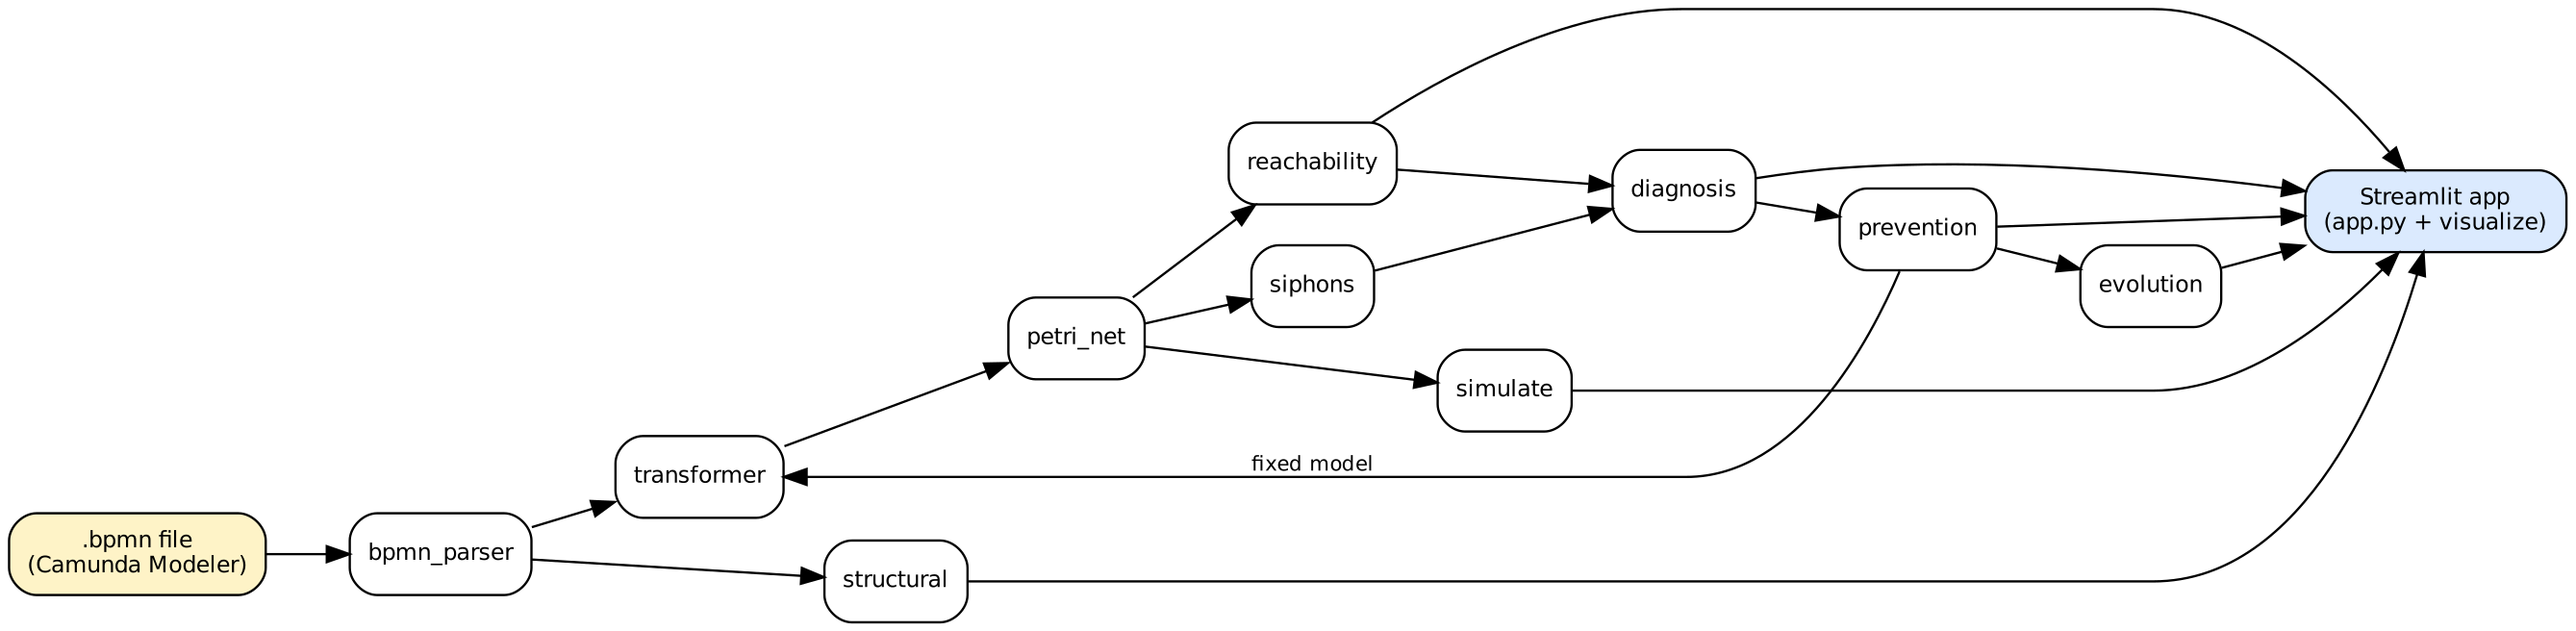
\includegraphics[width=\columnwidth]{architecture.png}}
\caption{Module structure of the tool.}
\label{fig:arch}
\end{figure}

\begin{table}[htbp]
\caption{Modules and Their Main Functions}
\begin{center}
\footnotesize
\begin{tabular}{|p{0.25\columnwidth}|p{0.63\columnwidth}|}
\hline
\textbf{Module} & \textbf{Purpose} \\
\hline
\texttt{bpmn\_parser} & reads the XML into nodes, flows and annotations \\
\texttt{transformer} & applies Table~\ref{tab:map}; mapping check \\
\texttt{petri\_net} & net structure and firing rule \\
\texttt{structural} & patterns P1--P6 \\
\texttt{reachability} & state space, dead markings, soundness, safeness \\
\texttt{diagnosis} & explanation of each dead marking \\
\texttt{siphons} & minimal and problem siphons \\
\texttt{prevention} & quick fixes, control places, permissiveness \\
\texttt{evolution} & insert, delete and replace operations \\
\texttt{simulate} & timed simulation with probabilities \\
\texttt{app.py} & Streamlit web interface \\
\hline
\end{tabular}
\label{tab:mod}
\end{center}
\end{table}

The web interface is built with Streamlit~\cite{streamlit}. A user picks one of the included models or uploads a
BPMN file, and moves through pages for the process model, the Petri net, the detection results, the cause and
fix, a token game in which transitions are fired by hand, and the simulation (Fig.~\ref{fig:ui}). BPMN diagrams
are drawn with bpmn-js~\cite{bpmnjs} and Petri nets with Graphviz in the browser, so nothing has to be installed
beyond two Python packages. The application is deployed at \url{https://bpm-deadlock.streamlit.app}. A suite of
58 automated tests checks the expected verdict, pattern and fix for every model.

\begin{figure}[htbp]
\centerline{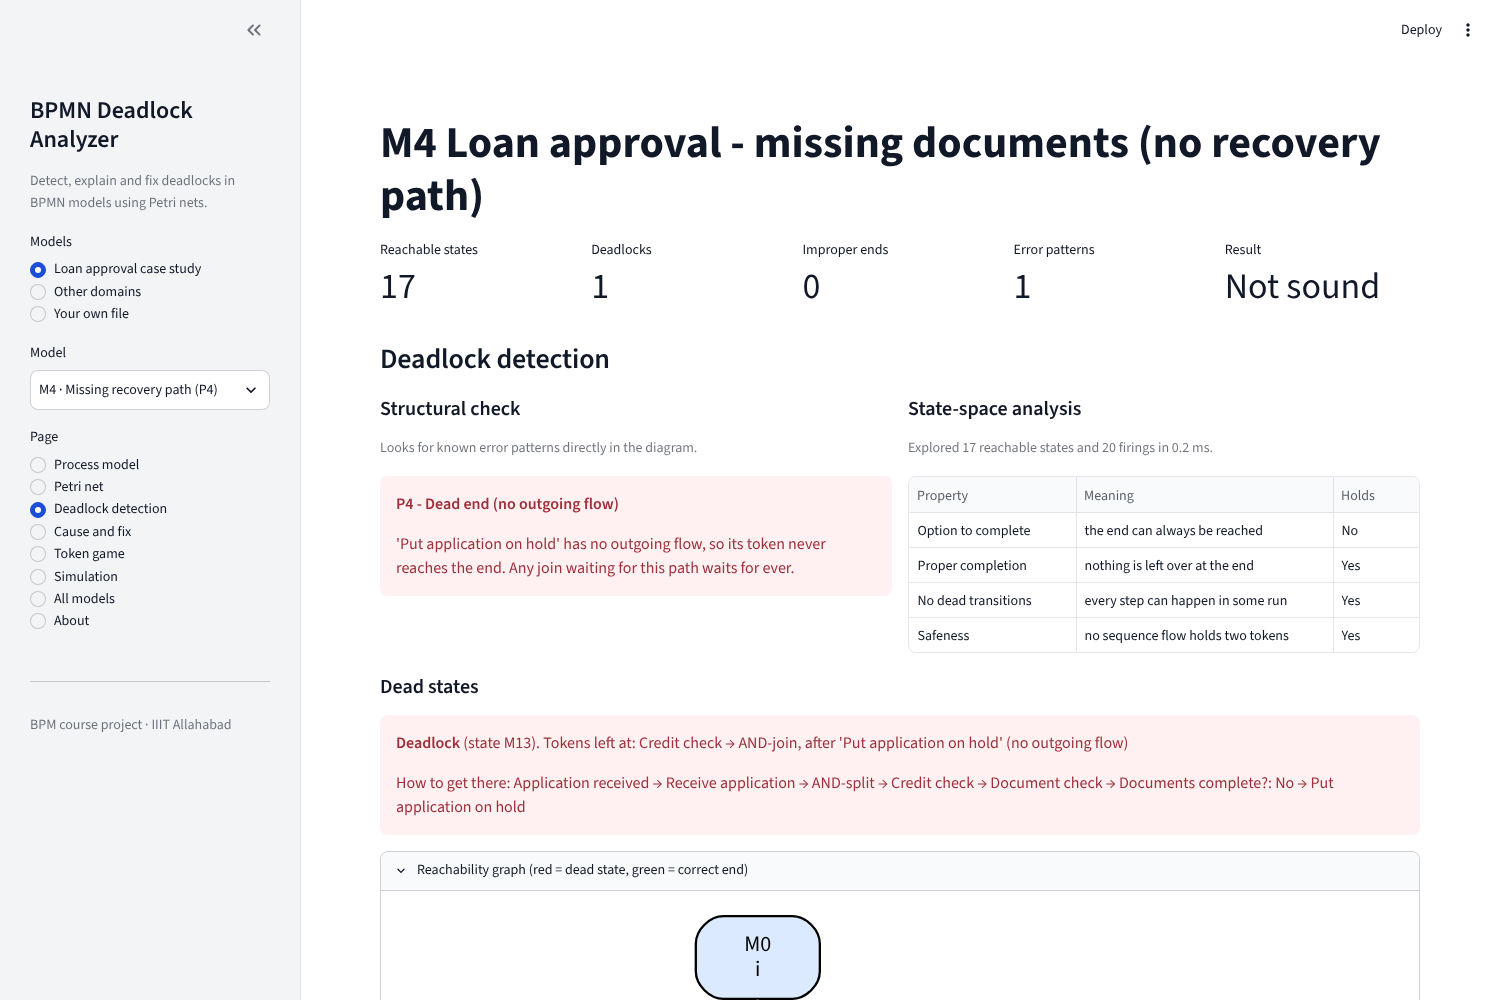
\includegraphics[width=\columnwidth]{ui_detect.png}}
\caption{Detection page of the web application for model M4.}
\label{fig:ui}
\end{figure}

\section{Case Study and Results}

\subsection{Models}
\begin{figure}[htbp]
\centerline{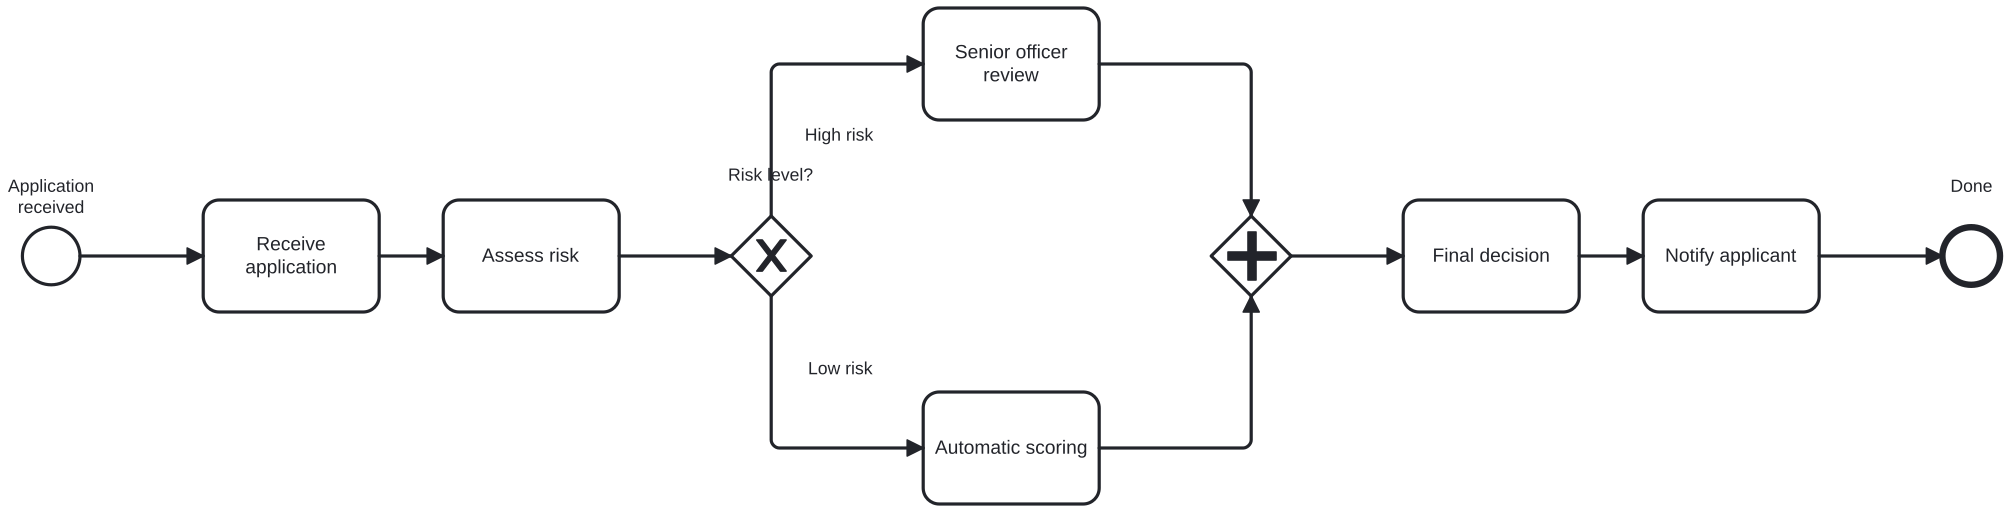
\includegraphics[width=\columnwidth]{bpmn_M3_wrong_join.png}}
\caption{M3: the XOR-split ``Risk level?'' is closed by an AND-join.}
\label{fig:m3}
\end{figure}

The dataset consists of 16 BPMN 2.0 models. Six describe a loan approval process of growing complexity:
\begin{itemize}
\item M1 is a sequence of four tasks.
\item M2 runs the credit check and the document check in parallel.
\item M3 routes the application by risk level with an XOR-split but closes the branches with an AND-join
(Fig.~\ref{fig:m3}).
\item M4 is the scenario from the introduction: the ``on hold'' task has no outgoing flow.
\item M5 runs a credit assessment and a fraud check in parallel. Both need the single loan officer and the
single credit-system session, and they take them in opposite orders.
\item M6 combines the corrected parts with durations, branch probabilities and a shared officer
(Fig.~\ref{fig:m6}).
\end{itemize}

\begin{figure*}[htbp]
\centerline{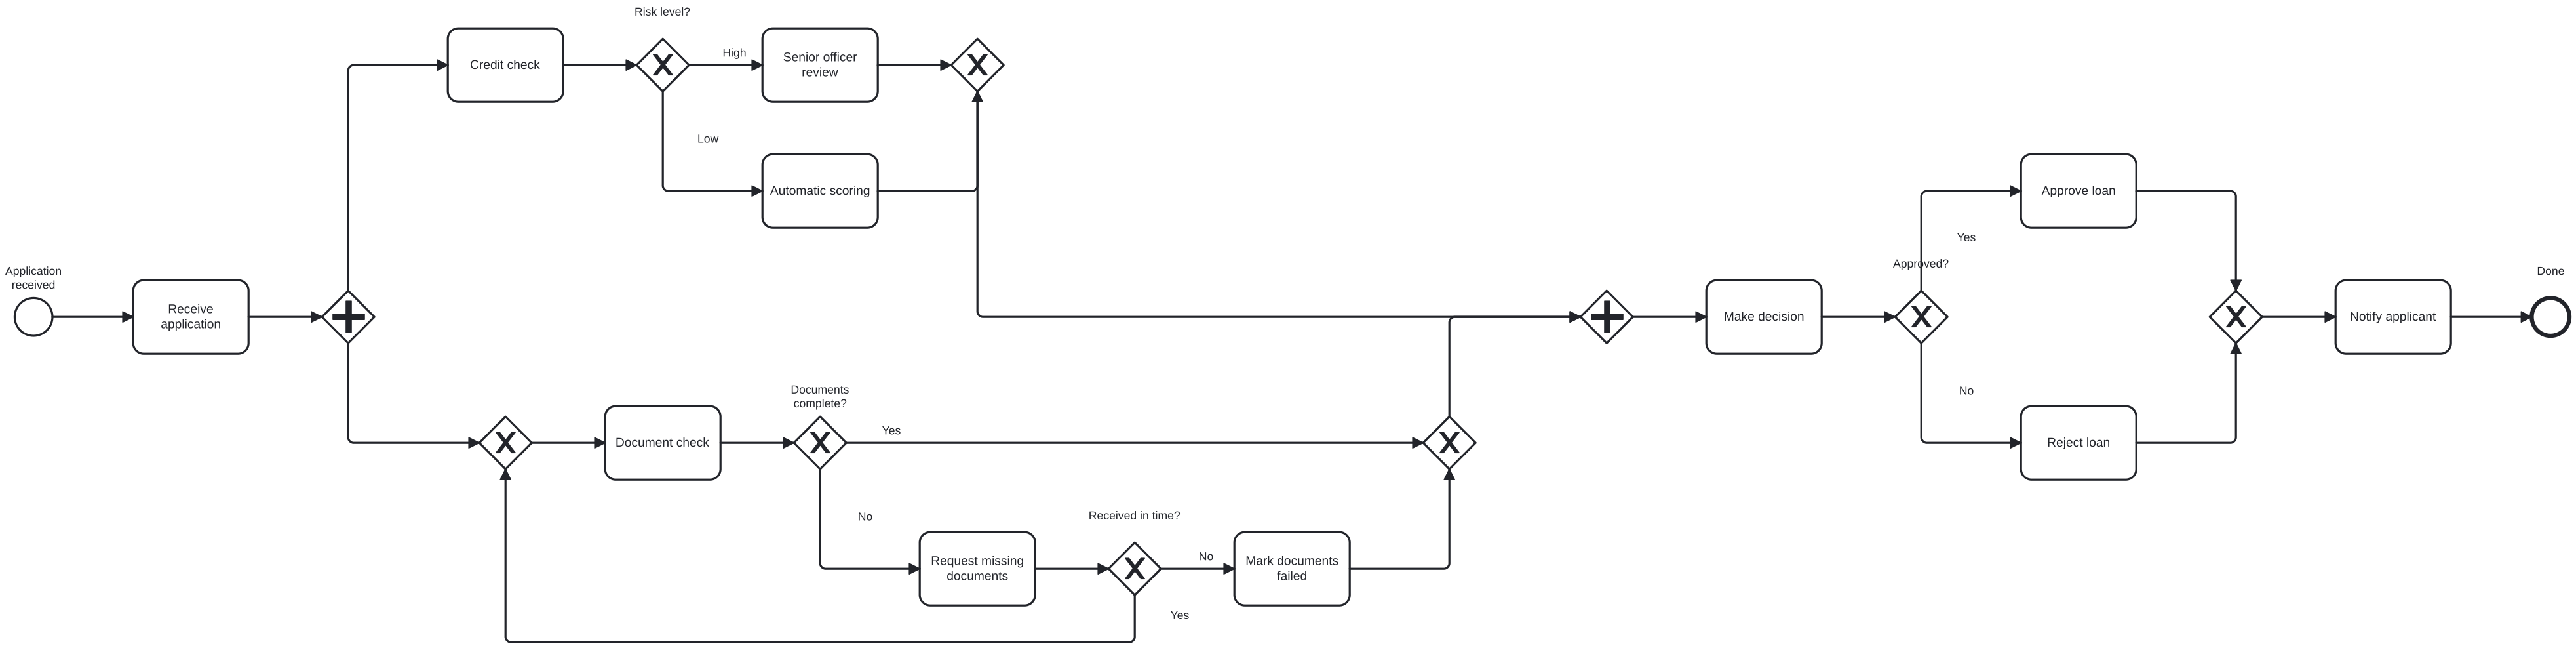
\includegraphics[width=0.95\textwidth]{bpmn_M6_full_timed.png}}
\caption{M6, the corrected loan approval model with resubmission loop, coordinated rejection and risk routing.}
\label{fig:m6}
\end{figure*}
C1 is a larger loan process with five defects, described in Section~VI-D. M3, M4, M5 and C1 each have a
hand-corrected version. Five further models come from other domains: order fulfilment (D1), an insurance claim
(D2), a leave request (D3), a hospital admission that needs a bed and a doctor (D4), and a purchase order with
a revision loop (D5).

\subsection{Detection and Correction}
Table~\ref{tab:res} summarises the faulty and the sound original models. Eight models are unsound: four
deadlock through control-flow errors, two through circular waits, D3 completes improperly, and C1 combines
both kinds.

\begin{table*}[htbp]
\caption{Analysis Results Before and After Correction (S = Reachable States, D = Deadlocks, I = Improper Completions)}
\begin{center}
\begin{tabular}{|l|r|r|r|r|r|c|c|c|l|c|r|}
\hline
\textbf{Model} & $|P|$ & $|T|$ & \textbf{S} & \textbf{D} & \textbf{I} & \textbf{Sound} & \textbf{Safe} &
\textbf{Pattern} & \textbf{Correction} & \textbf{Sound after} & \textbf{S after} \\
\hline
M1 sequential        & 7  & 6  & 7  & 0 & 0 & yes & yes & --  & --                                & --  & -- \\
M2 parallel          & 11 & 9  & 11 & 0 & 0 & yes & yes & --  & --                                & --  & -- \\
M3 wrong join        & 12 & 11 & 8  & 2 & 0 & no  & yes & P1  & AND-join to XOR-join              & yes & 12 \\
M4 missing recovery  & 14 & 12 & 17 & 1 & 0 & no  & yes & P4  & redesign (M4-fixed)               & yes & 32 \\
M5 resource deadlock & 17 & 13 & 20 & 1 & 0 & no  & yes & P6  & control place $V_1$               & yes & 19 \\
M6 full timed        & 30 & 31 & 82 & 0 & 0 & yes & yes & --  & --                                & --  & -- \\
C1 complex           & 40 & 36 & 32 & 3 & 0 & no  & yes & P1--P4, P6 & three rounds (Table~\ref{tab:c1}) & yes & 212 \\
\hline
D1 order fulfilment  & 13 & 12 & 13 & 0 & 0 & yes & yes & --  & --                                & --  & -- \\
D2 insurance claim   & 10 & 9  & 7  & 2 & 0 & no  & yes & P1  & AND-join to XOR-join              & yes & 10 \\
D3 leave request     & 10 & 9  & 25 & 0 & 1 & no  & no  & P3  & XOR-join to AND-join              & yes & 10 \\
D4 hospital admission& 16 & 12 & 19 & 1 & 0 & no  & yes & P6  & control place $V_1$               & yes & 18 \\
D5 purchase order    & 10 & 9  & 3  & 1 & 0 & no  & yes & P2  & AND-join to XOR-join              & yes & 10 \\
\hline
\end{tabular}
\label{tab:res}
\end{center}
\end{table*}

\textbf{M3.} Both dead markings hold one token in front of the AND-join. The trace
\emph{Receive application, Assess risk, Risk level?: High, Senior officer review} leaves the join waiting for
``Automatic scoring'', which was never started, and the low-risk path fails the same way. Pattern P1 names the
same two gateways. With an XOR-join the net is sound with 12 states.

\textbf{M4.} The dead marking has one token between ``Credit check'' and the AND-join and one in the stuck place
after ``Put application on hold'' (Fig.~\ref{fig:m4pn}). No change of gateway type can help, because the missing
token is never produced. The hand-corrected M4-fixed requests the missing documents and repeats the check; if
they do not arrive, the documents are marked as failed. Either way the AND-join receives a result, and a later
decision approves or rejects the loan. M4-fixed is sound with 32 states.

\begin{figure*}[htbp]
\centerline{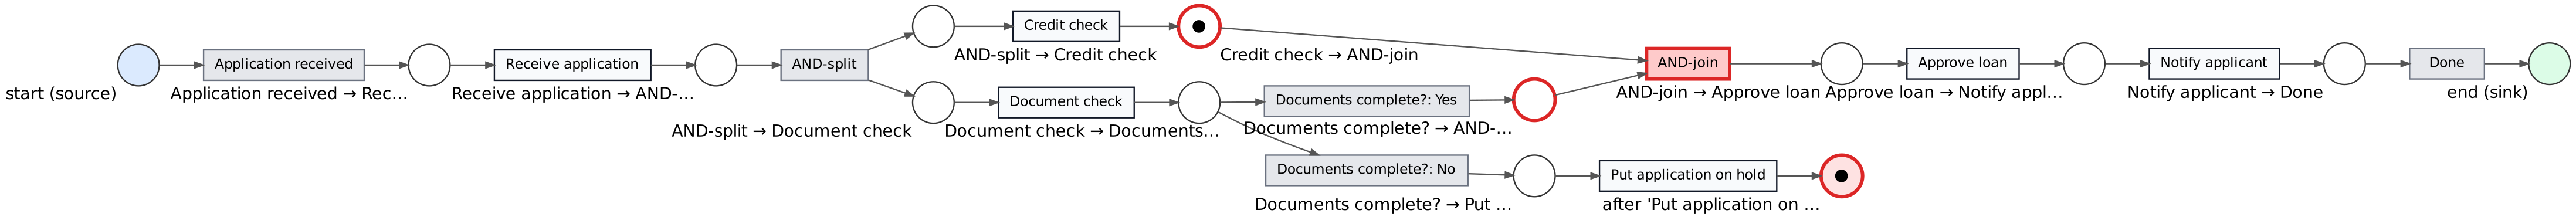
\includegraphics[width=0.92\textwidth]{pn_M4_missing_recovery_dead.png}}
\caption{Petri net of M4 in its dead marking. Red: the waiting AND-join, the empty place it needs and the stuck token.}
\label{fig:m4pn}
\end{figure*}

\textbf{M5.} The trace \emph{AND-split, Assign loan officer, Open credit system (fraud)} reaches a marking in
which each branch holds one resource and waits for the other. The siphon is
$S=\{r_{officer},r_{credit},p_5,p_8\}$, where $p_5$ and $p_8$ are the places in which a branch holds both
resources. $S$ holds two tokens in $M_0$ and none in the deadlock. The control place $V_1$ starts with one token.
The first resource request of each branch takes it, and the branch returns it when it releases both resources
(Fig.~\ref{fig:m5mon}). Only one branch can then hold resources at a time, and the net is sound with 19 states.
The hand-corrected M5-fixed, in which both branches take the officer first, is also sound. P6 finds the opposite
order directly in the diagram.

\begin{figure*}[htbp]
\centerline{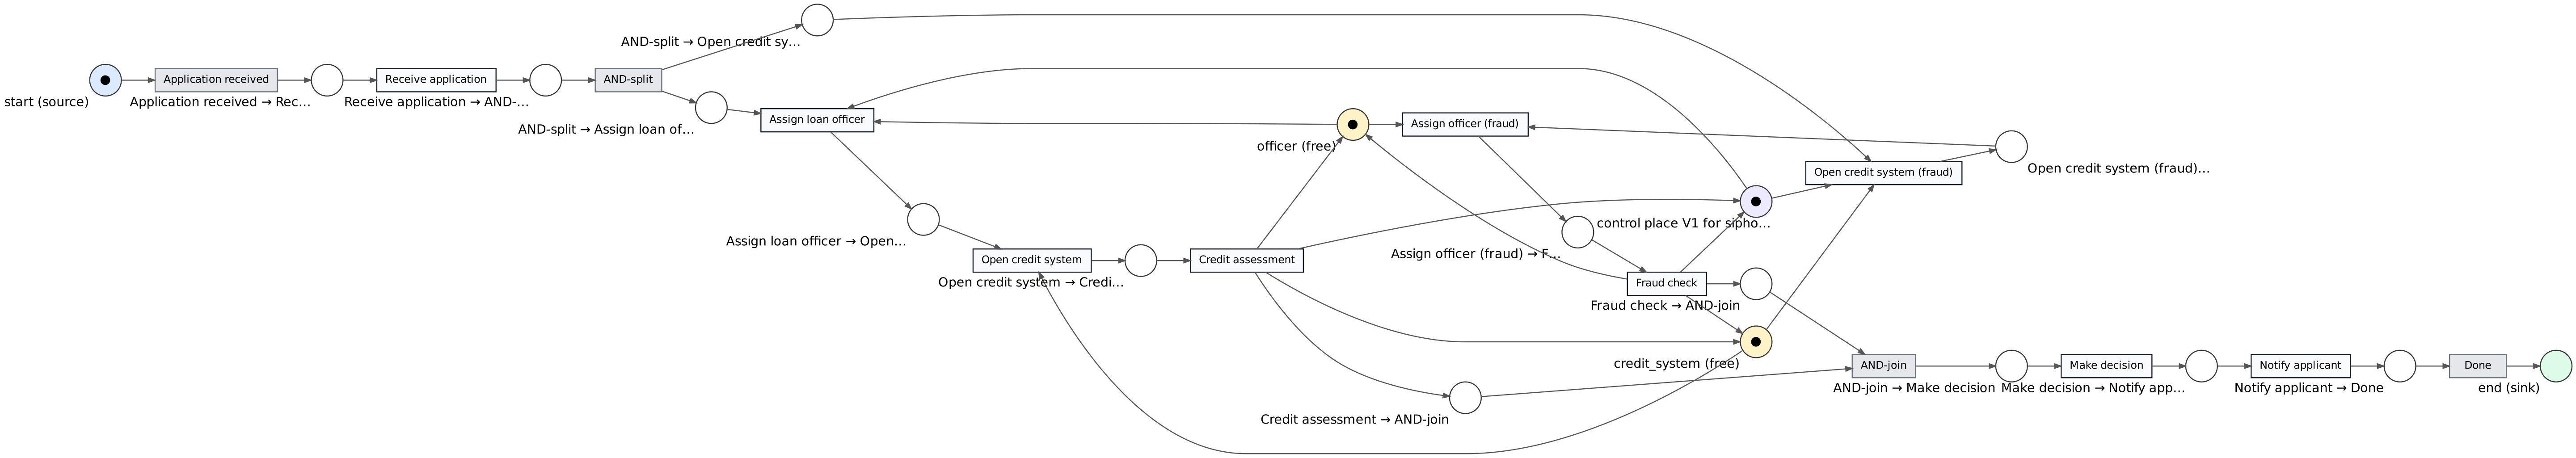
\includegraphics[width=0.92\textwidth]{pn_M5_monitored.png}}
\caption{M5 with the control place $V_1$ (purple) added by the prevention step.}
\label{fig:m5mon}
\end{figure*}

\textbf{Other domains.} D2 and D5 repeat P1 and P2. D3 is unsound without a deadlock: its XOR-join lets both
parallel branches through, so ``Update team calendar'' runs twice and two tokens reach the end. It is the only
model that is not safe, since both flows after the XOR-join can hold two tokens. D4 has the circular wait of
M5 with a bed and a doctor.

\subsection{Alternative Fixes and Permissiveness}
The split-side fixes of~\cite{kraeuter} are sound as well: an AND-split at ``Risk level?'' in M3 (12 states), an
AND-split at ``Claim size?'' in D2 (10 states) and an XOR-split in D3 (10 states). Each of them changes what the
business does; in M3, for example, every application would go through both reviews. The tool shows them but does
not apply them.

For the control places, the original M5 has 19 good states and the controlled net keeps all 19. In D4 it keeps
18 of 18. Both controllers are therefore maximally permissive, and all their arcs have weight one.

\subsection{A Complex Model with Several Defects}
C1 (Fig.~\ref{fig:c1}) is an end-to-end loan process with 30 BPMN elements and two shared resources, one loan
officer and one credit-system session. An AND-split starts three branches. The credit branch opens the credit
system, assigns the officer, assesses the application and routes it by risk level. The fraud branch needs the
same two resources. The document branch contains a resubmission loop. After the decision the case is approved,
rejected or referred to a manager, and the applicant is notified by e-mail and SMS in parallel before the case
is archived. We built in one defect of each kind the framework handles: (1)~the risk XOR-split is closed by an
AND-join (P1); (2)~the document loop is entered through an AND-join (P2); (3)~the fraud branch takes the officer
before the credit system, the opposite of the credit branch (P6); (4)~``Refer to manager'' has no outgoing flow
(P4); and (5)~the notifications are merged by an XOR-join (P3).

\begin{figure*}[htbp]
\centerline{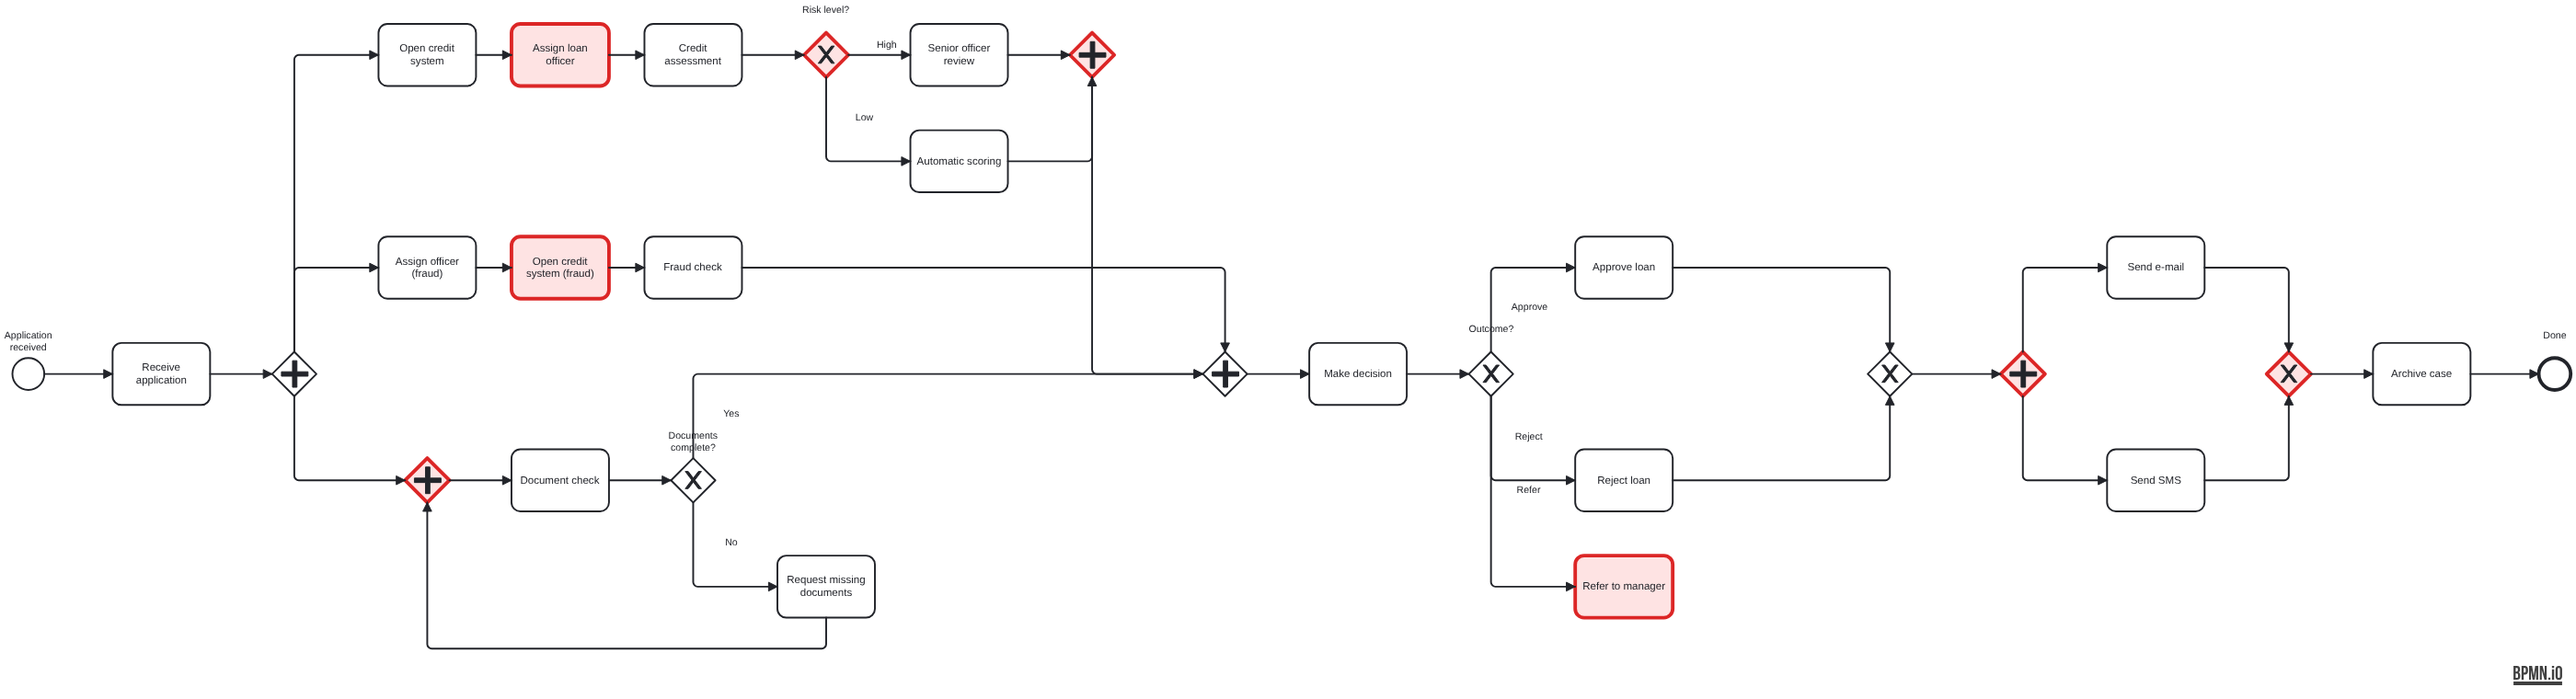
\includegraphics[width=\textwidth]{bpmn_C1_complex.png}}
\caption{C1, a loan process with five defects. The elements named by the structural check are outlined in red.}
\label{fig:c1}
\end{figure*}

The Petri net has 40 places and 36 transitions, and the mapping check finds no error. The structural check
reports all five patterns. The state-space analysis, however, finds only 32 states and 3 deadlocks. One is the
circular wait between the credit and the fraud branch. In the other two, one for each risk level, the risk
AND-join waits for the branch that was not chosen. All three contain a token in front of the loop-entry
AND-join, so the document branch never starts (Fig.~\ref{fig:c1pn}). Every run therefore stops before the
decision. The dead end after ``Refer to manager'' and the notification merge are never reached, and 23 of the
36 transitions are dead.

\begin{figure*}[htbp]
\centerline{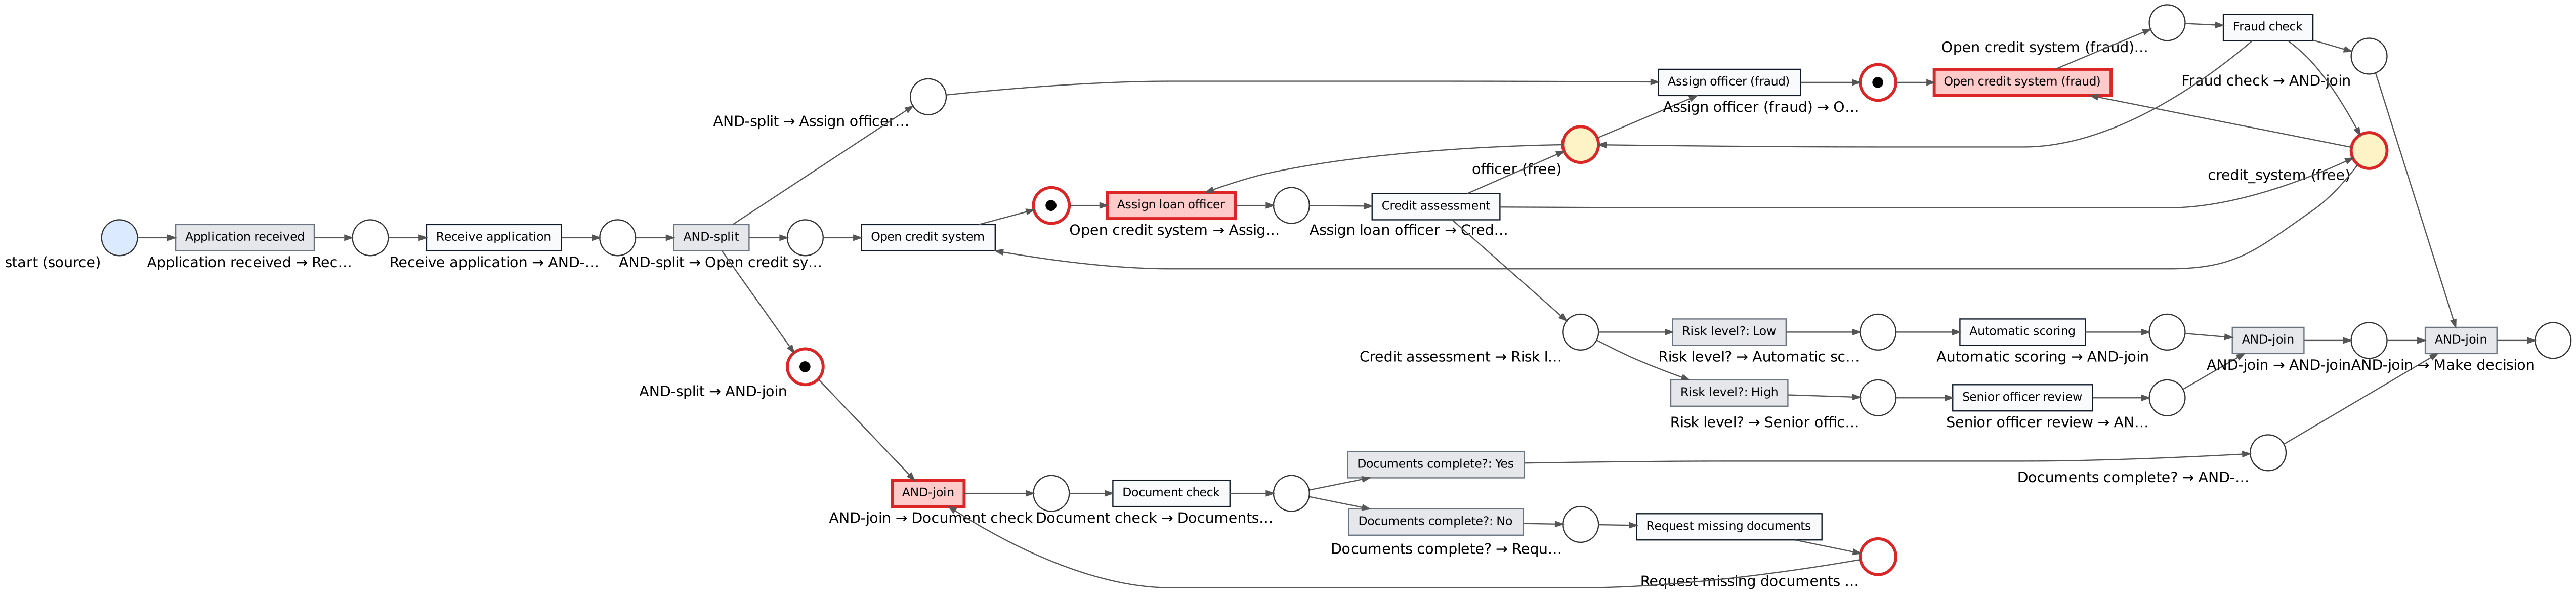
\includegraphics[width=\textwidth]{pn_C1_complex_dead_part.png}}
\caption{Petri net of C1 up to the main AND-join, in its first dead marking. The part after the join is never
reached. Red: the token before the loop-entry AND-join, the two branches that each hold one resource, and the
transitions waiting for the other resource or for the loop-back token.}
\label{fig:c1pn}
\end{figure*}

Table~\ref{tab:c1} shows the repair, one class of cause per round. Round~1 applies the three gateway fixes. Every
branch can now finish, the state space grows to 217 states and no transition is dead. The analysis now shows a
deadlock that was hidden before: the trace \emph{\ldots\ Outcome?: Refer, Refer to manager} ends with a token in
the stuck place. In round~2 the dead end is redesigned by hand: a ``Manager decision'' task leads the referred
case to the merge of the other outcomes. Only the circular wait remains. In round~3 the siphon
$\{r_{officer},r_{credit},p_5,p_{10}\}$ receives a control place $V_1$ with one token, taken by ``Open credit
system'' and ``Assign officer (fraud)'' and returned by ``Credit assessment'' and ``Fraud check''. The net is
then sound with 212 states. $V_1$ keeps all 212 good states of the round-2 net.

\begin{table}[htbp]
\caption{Round-by-Round Repair of C1 (S = States, D = Deadlocks, DT = Dead Transitions)}
\begin{center}
\begin{tabular}{|c|p{0.40\columnwidth}|r|r|r|c|}
\hline
\textbf{Round} & \textbf{Fix applied} & \textbf{S} & \textbf{D} & \textbf{DT} & \textbf{Sound} \\
\hline
0 & none & 32 & 3 & 23 & no \\
1 & gateway fixes P1, P2, P3 & 217 & 2 & 0 & no \\
2 & redesign of dead end P4 & 218 & 1 & 0 & no \\
3 & control place $V_1$ for P6 & 212 & 0 & 0 & yes \\
\hline
-- & C1-fixed (repair in BPMN) & 212 & 0 & 0 & yes \\
\hline
\end{tabular}
\label{tab:c1}
\end{center}
\end{table}

Instead of a control place, the hand-corrected C1-fixed takes the credit system first on both branches. It is
sound with the same 212 states. The change detection of~\cite{zhang} describes the repair from C1 to C1-fixed as
3 insert operations (the new task and its two flows) and 6 replace operations (three gateway types and the
three re-ordered flows of the fraud branch).

\subsection{Cross-Check and Running Time}
pm4py's WOFLAN check~\cite{pm4py} reads only the control flow, so we compared it with our analysis of the control
flow of each model. The verdicts agree on all 16 models. The state-space analysis takes at most 5~ms per model;
the complete pipeline, including the generation and re-analysis of every candidate fix, takes at most 68~ms.

\subsection{Scalability}
We generated the worst-case benchmark of~\cite{kraeuter}: an AND-split into $n$ branches of $m$ tasks each, whose
state space grows as $(m+1)^n$. Table~\ref{tab:bench} compares the number of states. Ours is theirs plus one in
every case, because our start event has its own transition, so the two encodings are equally compact. The
largest complete run, 9\,265 states, takes about 0.26~s in Python. At 15 parallel branches our search reaches its
limit of 20\,000 states and reports an inconclusive verdict.

\begin{table}[htbp]
\caption{Parallel-Branch Benchmark of~\cite{kraeuter} (Number of States)}
\begin{center}
\begin{tabular}{|r|r|r|r|l|}
\hline
\textbf{Branches} & \textbf{Length} & \textbf{Ours} & \textbf{\cite{kraeuter}} & \textbf{Our verdict} \\
\hline
5 & 1 & 36 & 35 & sound \\
10 & 1 & 1\,028 & 1\,027 & sound \\
5 & 3 & 1\,028 & 1\,027 & sound \\
5 & 5 & 7\,780 & 7\,779 & sound \\
3 & 10 & 1\,335 & 1\,334 & sound \\
3 & 20 & 9\,265 & 9\,264 & sound \\
15 & 1 & $\ge$20\,000 & 32\,771 & inconclusive \\
\hline
\end{tabular}
\label{tab:bench}
\end{center}
\end{table}

\subsection{Simulation}
M6 contains the assumed durations and probabilities, for example 30\% high-risk applications,
25\% incomplete documents and an 80\% chance that requested documents arrive. All 1\,000 simulated cases
complete. The mean cycle time is 62.4 minutes, the median 50 minutes and the 90th percentile 78 minutes
(Fig.~\ref{fig:sim}). The distribution has separate peaks because the slow paths, a senior review or a round of
document requests, add a fixed amount of time. For the uncorrected M5 with both branches starting together, none
of the 1\,000 cases completes; with the control place, all of them do.

\begin{figure}[htbp]
\centerline{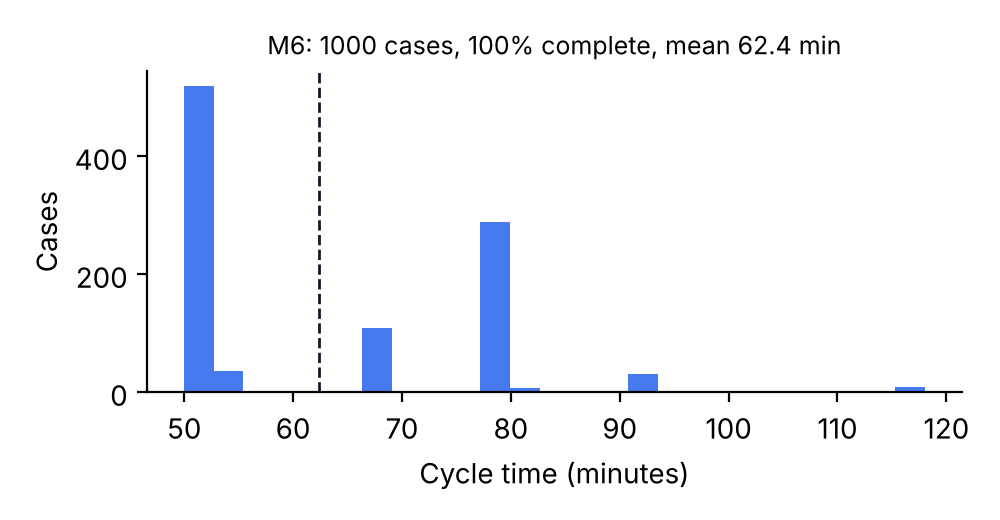
\includegraphics[width=\columnwidth]{sim_M6.png}}
\caption{Cycle times of 1\,000 simulated cases of M6.}
\label{fig:sim}
\end{figure}

\section{Discussion}
C1 shows why the framework re-analyses after every fix. When a model has several defects, the state space only
contains the defects that a run reaches first. The others sit behind dead transitions and produce no dead
marking of their own until the earlier ones are fixed. The structural check found all five defects at once
because it does not depend on reachability. The two methods therefore do different jobs: the structural check
names the suspicious elements quickly, and the state-space analysis confirms each problem with a concrete trace
and proves the corrected model sound. The structural check is a heuristic. It can miss errors in shapes that
none of the six patterns describes, and in unusual structures it can raise a false alarm.

The corrections keep the behaviour that worked. In our models, every run that completed before a gateway fix
still completes after it. A control place does not remove any activity; it only delays one branch until the
other has released its resources. The permissiveness measure makes this checkable: in M5, D4 and C1 no good
state was lost.

The work has clear limits. OR-joins are treated like XOR-joins. Sub-processes, pools, message flows and boundary
events are not translated; the hierarchical mapping of~\cite{zhang} covers several of them. Each model is
analysed for a single case, so conflicts between two loan applications that share an officer are outside the
analysis. Problem siphons are taken from the state space instead of the mixed-integer program of~\cite{wang},
which would be needed for nets too large to explore. The durations and probabilities in M6 are assumed, not
measured. The repair of a dead end (P4) cannot be automated, because it requires a business decision about what
should happen to the case.

\section{Conclusion and Future Work}
Petri nets turned out to be a practical way to detect, explain and prevent deadlocks in BPMN models. The tool
found every injected error in the 16 models and named the responsible elements. Six of the eight faulty models
were repaired automatically; M4 and the dead end in C1 each needed one manual change. Every repair was verified as
sound. In the complex model the
round-by-round repair uncovered two defects that the first analysis could not see. The control places were
maximally permissive in all three resource cases.

Three extensions follow from the work we build on. Coloured tokens, as in~\cite{zhang}, would let several cases
run in one net, so that resource conflicts between loan applications can be found. The mixed-integer siphon
detection of~\cite{wang} would remove the need for the full state space in large nets. Replaying the witness
trace on the BPMN diagram itself, as in~\cite{kraeuter}, would make the explanation easier to follow for people
who do not read Petri nets.

\section*{Acknowledgment}
% Draft acknowledgment: keep, edit or remove it according to your course's policy.
We thank the course instructor and teaching assistant of the Business Process Management course for their
feedback, in particular the suggestions to build on recent literature and to study a model with several
interacting defects. An AI assistant (Claude, by Anthropic) helped with parts of the implementation and with
drafting this report; the authors checked all results and are responsible for the content.

\begin{thebibliography}{00}
\bibitem{kraeuter} T. Kr\"auter, P. St\"unkel, A. Rutle, H. K\"onig, and Y. Lamo, ``Instantaneous,
comprehensible, and fixable soundness checking of realistic BPMN models,'' 2024, arXiv:2407.03965. [Online].
Available: https://arxiv.org/abs/2407.03965
\bibitem{zhang} Z. Zhang, F. Ni, J. Liu, N. Chen, and X. Zhou, ``Collaborative modeling of BPMN and HCPN: Formal
mapping and iterative evolution of process models for scenario changes,'' Information, vol. 16, no. 4, Art. no.
323, 2025, doi: 10.3390/info16040323.
\bibitem{wang} S. G. Wang, X. Guo, O. Karoui, M. C. Zhou, D. You, and A. Abusorrah, ``A refined siphon-based
deadlock prevention policy for a class of Petri nets,'' IEEE Trans. Syst., Man, Cybern.: Syst., vol. 53, no. 1,
pp. 191--203, Jan. 2023, doi: 10.1109/TSMC.2022.3174421.
\bibitem{aalst} W. M. P. van der Aalst, ``The application of Petri nets to workflow management,'' J. Circuits,
Syst. Comput., vol. 8, no. 1, pp. 21--66, 1998.
\bibitem{murata} T. Murata, ``Petri nets: Properties, analysis and applications,'' Proc. IEEE, vol. 77, no. 4,
pp. 541--580, Apr. 1989.
\bibitem{bpmn} Object Management Group, ``Business Process Model and Notation (BPMN), version 2.0,'' 2011.
\bibitem{pm4py} A. Berti, S. J. van Zelst, and W. M. P. van der Aalst, ``Process mining for Python (PM4Py):
Bridging the gap between process- and data science,'' in Proc. ICPM Demo Track, 2019, pp. 13--16.
\bibitem{streamlit} Streamlit, ``Streamlit: A faster way to build and share data apps,'' software. [Online].
Available: https://streamlit.io
\bibitem{bpmnjs} bpmn.io, ``bpmn-js: A BPMN 2.0 rendering toolkit and web modeler,'' software. [Online].
Available: https://github.com/bpmn-io/bpmn-js
\end{thebibliography}

\end{document}
